\documentclass[conference]{IEEEtran}
\IEEEoverridecommandlockouts

\usepackage{iftex}
\ifXeTeX
  % XeLaTeX/Tectonic: TeX Gyre Termes là bản Times có đủ dấu tiếng Việt cho tên tác giả.
  \usepackage{fontspec}
  \setmainfont{texgyretermes}[Extension=.otf, UprightFont=*-regular, BoldFont=*-bold,
    ItalicFont=*-italic, BoldItalicFont=*-bolditalic]
\else
  \usepackage[T5,T1]{fontenc}
  \usepackage[utf8]{inputenc}
\fi
\usepackage{cite}
\usepackage{amsmath,amssymb}
\usepackage{graphicx}
\usepackage{booktabs}
\usepackage{xcolor}
\usepackage{tikz}
\usetikzlibrary{positioning,arrows.meta,decorations.pathreplacing,calc}
\usepackage{url}
\usepackage[hidelinks]{hyperref}

\graphicspath{{figures/}}

\begin{document}

\title{Revisiting BERT+BiLSTM for IMDb Sentiment Classification: A Clean Reproduction and Head--Tail Fine-Tuning}

\author{
\IEEEauthorblockN{Vũ Quốc Đạt}
\IEEEauthorblockA{DE200522\\
\textit{FPT University}\\
Da Nang, Vietnam}
\and
\IEEEauthorblockN{Nguyễn Gia Phúc}
\IEEEauthorblockA{DE200407\\
\textit{FPT University}\\
Da Nang, Vietnam}
\and
\IEEEauthorblockN{Ngô Ngọc Trường Sơn}
\IEEEauthorblockA{DE200399\\
\textit{FPT University}\\
Da Nang, Vietnam}
}

\maketitle

\begin{abstract}
A recent study combined a frozen BERT encoder with a bidirectional LSTM (BiLSTM) for movie-review sentiment classification and reported 97.67\% accuracy on IMDb. That figure was obtained after merging the official training and test sets and re-splitting them, so it is not comparable with results on the standard test set. We reproduce the method on a leakage-controlled split of the full IMDb corpus that keeps the official 25{,}000-review test set intact, and evaluate every configuration with three random seeds. Following the authors' released code yields a test Macro-F1 of 89.41\%$\pm$0.67, and following the hyper-parameters described in the paper yields 84.97\%$\pm$0.30. We show that the main weakness of the original pipeline is truncation: 40\% of test reviews exceed 256 tokens, and the cut removes the end of the review, where reviewers often state their verdict. Keeping both the beginning and the end of each review raises a frozen BiLSTM from 90.14\% to 91.87\%, with almost all of the gain on truncated reviews. Fine-tuning the whole encoder on 128 head plus 382 tail tokens reaches 94.38\%$\pm$0.17 with BERT-base and 96.74\%$\pm$0.04 with RoBERTa-large, 7.33 points above the reproduced baseline. A movie-clustered paired bootstrap with Holm correction and per-seed McNemar tests confirms that each improvement is statistically significant. With RoBERTa-large, reviews longer than 512 tokens are classified as accurately as short ones.
\end{abstract}

\begin{IEEEkeywords}
sentiment analysis, BERT, RoBERTa, BiLSTM, reproducibility, long-text classification, IMDb
\end{IEEEkeywords}

\section{Introduction}
Binary sentiment classification of movie reviews is a standard benchmark for text classifiers, and the Large Movie Review Dataset (IMDb) introduced by Maas \textit{et al.}~\cite{maas2011} is its most widely used instance. Pre-trained transformers such as BERT~\cite{devlin2019} and RoBERTa~\cite{liu2019roberta} have pushed accuracy on this benchmark well above earlier word-vector and recurrent models. Nkhata \textit{et al.}~\cite{nkhata2023} proposed to feed the token representations of a frozen BERT encoder into a bidirectional LSTM~\cite{hochreiter1997,schuster1997} and reported 97.67\% accuracy on IMDb.

Two practical issues make that number hard to interpret. First, the released code merges the official IMDb training and test sets and draws a new random split, so the reported accuracy is not measured on the standard test set and cannot be compared directly with other work. Second, the paper and the code describe different settings (sequence length, learning rate and number of epochs), so it is not clear which configuration produced the reported result.

This paper makes three contributions:
\begin{itemize}
\item We build a leakage-controlled split of all 50{,}000 labeled IMDb reviews that preserves the official test set, and we reproduce both the code and the paper configurations of the BERT+BiLSTM method with three seeds each.
\item We identify truncation of long reviews as the dominant source of error in the original pipeline, and we quantify how much of it is removed by keeping the head and the tail of each review~\cite{sun2019}.
\item We show that full fine-tuning with head--tail inputs of 512 tokens lifts test Macro-F1 from 89.41\% to 94.38\% with BERT-base and to 96.74\% with RoBERTa-large, and we support every comparison with a movie-clustered bootstrap and McNemar tests.
\end{itemize}

\section{Related Work}
\textit{Sentiment classification on IMDb.} Maas \textit{et al.}~\cite{maas2011} released 50{,}000 labeled reviews, balanced between positive and negative, together with a fixed train/test split of 25{,}000 reviews each. The split guarantees that no movie appears in both halves, so that a model cannot benefit from memorizing movie-specific vocabulary. Early neural approaches on this benchmark used convolutional~\cite{kim2014} and hierarchical attention networks~\cite{yang2016han}, which read a document as a sequence of sentences. Transfer learning changed the picture: ULMFiT~\cite{howard2018} showed that fine-tuning a pre-trained language model on the target domain substantially reduces the error on IMDb, and pre-trained transformers have since become the standard starting point.

\textit{Pre-trained encoders.} BERT~\cite{devlin2019} learns bidirectional contextual representations with masked language modeling. RoBERTa~\cite{liu2019roberta} keeps the architecture but trains longer, on more data, with dynamic masking and without the next-sentence objective, and usually transfers better to downstream classification. Both models can be used either as frozen feature extractors, with a task-specific head trained on top, or fine-tuned end to end. Fine-tuning updates all encoder weights and generally performs better, at a higher training cost.

\textit{Long documents.} Both encoders accept at most 512 tokens. Sun \textit{et al.}~\cite{sun2019} compared truncation strategies for fine-tuning BERT on long reviews and found that keeping the first 128 and the last 382 tokens worked best on IMDb, better than keeping only the head, only the tail, or pooling over chunks. Hierarchical models split a document into chunks, encode each chunk and combine the chunk representations with a recurrent or transformer layer~\cite{pappagari2019}, while sparse-attention models such as Longformer~\cite{beltagy2020} extend the input length directly. We adopt the simple head--tail strategy, which needs no architectural change.

\textit{BERT with recurrent heads.} Nkhata \textit{et al.}~\cite{nkhata2023} keep BERT frozen and train a BiLSTM over its token states. This reduces the number of trainable parameters but prevents the encoder from adapting to the task.

\textit{Reproducibility.} Reported improvements in NLP are often sensitive to random seeds, hyper-parameter budgets and data splits. Dodge \textit{et al.}~\cite{dodge2019} argue that results should be reported with their variance and computational budget. Following this advice, we report every configuration with three seeds, describe all deviations from the original code, and test differences statistically.

\section{Data and Evaluation Protocol}

\subsection{Leakage-controlled split}
We use all 50{,}000 labeled reviews of IMDb, without genre filtering and without the unlabeled portion. The official test set of 25{,}000 reviews (3{,}581 movies, 12{,}500 per class) is kept unchanged. From the official training set we remove 223 reviews: 98 exact duplicates within the training set, 123 reviews whose text also appears in the test set, and 2 reviews of a movie that also appears in the test set. The remaining reviews are split by movie into training and validation sets, so that no movie is shared between any two sets (Table~\ref{tab:data}). All model selection uses the validation set; the test set is used once per run.

\begin{table}[t]
\caption{Data split used in all experiments}
\label{tab:data}
\centering
\begin{tabular}{lrrrr}
\toprule
Split & Reviews & Movies & Negative & Positive \\
\midrule
Train & 21{,}027 & 2{,}910 & 10{,}467 & 10{,}560 \\
Validation & 3{,}750 & 514 & 1{,}867 & 1{,}883 \\
Test (official) & 25{,}000 & 3{,}581 & 12{,}500 & 12{,}500 \\
\bottomrule
\end{tabular}
\end{table}

\subsection{Review length}
IMDb reviews are long relative to the input limit of the encoders. With the BERT tokenizer, 87.4\% of test reviews exceed 128 tokens, 40.1\% exceed 256 tokens and 12.3\% (3{,}086 reviews) exceed 512 tokens. With the RoBERTa tokenizer, 2{,}940 test reviews (11.8\%) exceed 512 tokens. We call a review \emph{truncated} if it does not fit the input length of the model under evaluation, and we report results separately for truncated and short reviews. Table~\ref{tab:trunc} shows that the proportions are similar across the three splits, so the validation set is a faithful proxy for the test set in this respect.

\begin{table}[t]
\caption{Reviews longer than the input limit, per split}
\label{tab:trunc}
\centering
\footnotesize
\setlength{\tabcolsep}{4pt}
\begin{tabular}{lrrr}
\toprule
Input limit (tokenizer) & Train & Validation & Test \\
\midrule
128 (BERT) & 88.1\% & 87.1\% & 87.4\% \\
256 (BERT) & 41.1\% & 41.8\% & 40.1\% \\
512 (BERT) & 13.2\% & 14.1\% & 12.3\% \\
512 (RoBERTa) & 12.5\% & 13.4\% & 11.8\% \\
\bottomrule
\end{tabular}
\end{table}

\subsection{Metrics and repetitions}
The primary metric is Macro-F1 on the test set, the unweighted mean of the per-class F1 scores,
\begin{equation}
\mathrm{F1}_{\mathrm{macro}} = \frac{1}{2}\sum_{c\in\{\mathrm{neg},\mathrm{pos}\}} \frac{2\,P_c R_c}{P_c + R_c},
\end{equation}
where $P_c$ and $R_c$ are the precision and recall of class $c$; because the test set is balanced, mean accuracy and mean Macro-F1 differ by at most 0.03 points for every configuration we report. Each configuration is trained with seeds 42, 43 and 44, and we report the mean and the sample standard deviation over the three runs.

\subsection{Statistical testing}
Reviews of the same movie are not independent, so we test differences with a paired bootstrap that resamples \emph{movies} rather than reviews~\cite{efron1993}. In each of $B=10{,}000$ resamples we draw 3{,}581 test movies with replacement, take all reviews of the drawn movies, and compute
\begin{equation}
\Delta^{*}_{b} = \frac{1}{3}\sum_{s\in\{42,43,44\}} \Bigl(\mathrm{F1}_{\mathrm{macro}}^{(b)}(A_s) - \mathrm{F1}_{\mathrm{macro}}^{(b)}(C_s)\Bigr),
\end{equation}
where $A_s$ and $C_s$ are the predictions of the two compared systems trained with seed $s$. The 95\% confidence interval is the percentile interval of these differences. The two-sided $p$-value is computed with the usual add-one correction, so its smallest attainable value is $2/10{,}001 \approx 2\times10^{-4}$. Because we perform eight comparisons, the $p$-values are adjusted with the Holm procedure~\cite{holm1979}; the smallest attainable adjusted value is therefore 0.0016. As a complementary test, we apply the exact McNemar test~\cite{mcnemar1947,dietterich1998} to the paired predictions of each seed.

\section{Methods}

\subsection{Reproduction of BERT+BiLSTM}
The original model passes the token states of a frozen \texttt{bert-base-uncased} encoder through dropout ($p=0.5$) and a BiLSTM with 768 units per direction, followed by a two-way softmax layer. We re-implemented the model in PyTorch~\cite{paszke2019} and Hugging Face Transformers~\cite{wolf2020} and reproduced two configurations:
\begin{itemize}
\item \textit{Code configuration:} the first 256 tokens, Adam with learning rate $10^{-4}$ and decay $10^{-5}$, batch size 32, and four Keras epochs over a training set repeated twice (eight passes). As in the released code, the BiLSTM also reads padding positions, and the final model is evaluated without checkpoint selection.
\item \textit{Paper configuration:} the first 128 tokens, Adam with learning rate $3\times10^{-5}$, batch size 32 and ten epochs, as stated in the experimental section of the paper.
\end{itemize}
Table~\ref{tab:repro} contrasts the two configurations. Fig.~\ref{fig:arch}(a) shows the architecture.

\begin{table}[t]
\caption{Settings of the two reproduced configurations}
\label{tab:repro}
\centering
\footnotesize
\setlength{\tabcolsep}{4pt}
\begin{tabular}{lcc}
\toprule
Setting & Paper (as described) & Author code \\
\midrule
Input tokens (head only) & 128 & 256 \\
Optimizer & Adam & Adam \\
Learning rate & $3\times10^{-5}$ & $10^{-4}$ (decay $10^{-5}$) \\
Training & 10 epochs & 4 epochs $\times$ 2 repeats \\
Batch size & 32 & 32 \\
Encoder & frozen & frozen \\
BiLSTM over padding & yes & yes \\
Model evaluated & final & final \\
\bottomrule
\end{tabular}
\end{table}

\begin{figure*}[t]
\centering
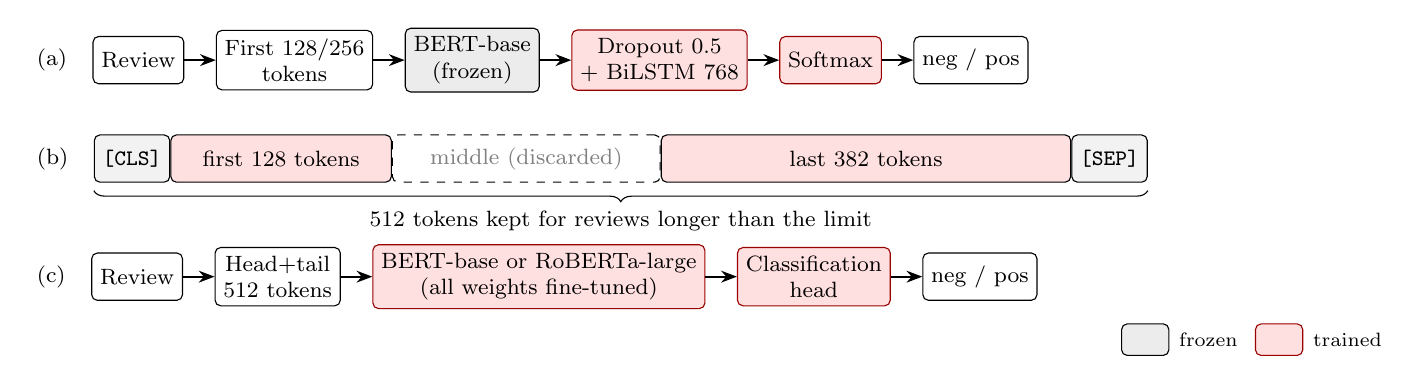
\begin{tikzpicture}[
  font=\footnotesize,
  box/.style={draw, rounded corners=2pt, minimum height=6mm, inner sep=3pt, align=center},
  frozen/.style={box, fill=gray!15},
  train/.style={box, fill=red!12, draw=red!60!black},
  arr/.style={-{Stealth[length=2mm]}, thick}]
% (a) original pipeline
\node[anchor=west] (la) at (0,0) {(a)};
\node[box, right=2mm of la] (a1) {Review};
\node[box, right=4mm of a1] (a2) {First 128/256\\tokens};
\node[frozen, right=4mm of a2] (a3) {BERT-base\\(frozen)};
\node[train, right=4mm of a3] (a4) {Dropout 0.5\\+ BiLSTM 768};
\node[train, right=4mm of a4] (a5) {Softmax};
\node[box, right=4mm of a5] (a6) {neg / pos};
\foreach \u/\v in {a1/a2,a2/a3,a3/a4,a4/a5,a5/a6} \draw[arr] (\u) -- (\v);
% (b) head--tail selection
\node[anchor=west] (lb) at (0,-1.25) {(b)};
\node[box, minimum width=6mm, right=2mm of lb, fill=gray!10] (cls) {\texttt{[CLS]}};
\node[box, minimum width=28mm, right=0mm of cls, fill=red!12] (head) {first 128 tokens};
\node[box, minimum width=34mm, right=0mm of head, dashed, text=gray] (mid) {middle (discarded)};
\node[box, minimum width=52mm, right=0mm of mid, fill=red!12] (tail) {last 382 tokens};
\node[box, minimum width=6mm, right=0mm of tail, fill=gray!10] (sep) {\texttt{[SEP]}};
\draw[decorate, decoration={brace, amplitude=4pt, mirror}] ([yshift=-1mm]cls.south west) -- node[below=4pt] {512 tokens kept for reviews longer than the limit} ([yshift=-1mm]sep.south east);
% (c) fine-tuned pipeline
\node[anchor=west] (lc) at (0,-2.75) {(c)};
\node[box, right=2mm of lc] (c1) {Review};
\node[box, right=4mm of c1] (c2) {Head+tail\\512 tokens};
\node[train, right=4mm of c2] (c3) {BERT-base or RoBERTa-large\\(all weights fine-tuned)};
\node[train, right=4mm of c3] (c4) {Classification\\head};
\node[box, right=4mm of c4] (c5) {neg / pos};
\foreach \u/\v in {c1/c2,c2/c3,c3/c4,c4/c5} \draw[arr] (\u) -- (\v);
\node[frozen, minimum height=4mm, minimum width=6mm, label={[font=\scriptsize]right:frozen}] at (14.2,-3.55) {};
\node[train, minimum height=4mm, minimum width=6mm, label={[font=\scriptsize]right:trained}] at (15.9,-3.55) {};
\end{tikzpicture}
\caption{Pipelines compared in this paper. (a) BERT+BiLSTM of~\cite{nkhata2023} with a frozen encoder and head-only truncation. (b) Head--tail input selection~\cite{sun2019}. (c) Full fine-tuning with head--tail inputs.}
\label{fig:arch}
\end{figure*}

Our reproduction differs from the released code in four documented ways: it uses the leakage-controlled split instead of a re-split of train and test; it runs in PyTorch with a BF16 encoder; it shuffles the whole training set every pass instead of using a small shuffle buffer; and it matches predictions with labels by review identifier, which avoids an ordering problem in the original evaluation script.

\subsection{Frozen-encoder baselines}
To separate the effect of the classification head from the effect of input selection, we train three heads on top of the same frozen BERT-base encoder with 256-token inputs: masked mean pooling followed by a linear layer, a BiLSTM over the first 256 tokens, and the same BiLSTM over a head--tail selection that keeps the first 127 and the last 127 content tokens of reviews that are too long. These baselines use AdamW~\cite{loshchilov2019} with learning rate $10^{-4}$, weight decay 0.01, an effective batch size of 32, BiLSTM hidden size 768 and dropout 0.5. They are trained for 50 epochs, and the checkpoint with the best validation Macro-F1 is evaluated on the test set.

\subsection{Head--tail fine-tuning}
Formally, let a review be tokenized into content tokens $x_1,\dots,x_n$ and let $L$ be the number of content positions available after the special tokens. The input is
\begin{equation}
\mathrm{sel}(x) =
\begin{cases}
(x_1,\dots,x_n) & n \le L,\\
(x_1,\dots,x_h,\; x_{n-t+1},\dots,x_n) & n > L,
\end{cases}
\end{equation}
with $h+t=L$ (Fig.~\ref{fig:arch}b). For the fine-tuned models $L=510$, $h=128$ and $t=382$; for the frozen head--tail baseline $L=254$ and $h=t=127$.

Our main models fine-tune all encoder weights together with the standard sequence-classification head of Hugging Face Transformers, which operates on the representation of the first token. Reviews longer than the limit keep the first 128 and the last 382 tokens, which together with the two special tokens fill the 512-token input~\cite{sun2019}. We fine-tune BERT-base (110M parameters) and RoBERTa-large (355M parameters) under the same protocol (Table~\ref{tab:hparams}): AdamW with weight decay 0.01, linear warm-up over the first 10\% of steps followed by linear decay to zero, gradient clipping at 1.0, BF16 autocast with FP32 master weights, three epochs, and selection of the epoch with the best validation Macro-F1. RoBERTa-large uses a smaller learning rate, which is customary for large encoders, and gradient checkpointing~\cite{chen2016} together with per-tensor optimizer updates so that training fits in 8~GB of GPU memory.

\begin{table}[t]
\caption{Fine-tuning hyper-parameters}
\label{tab:hparams}
\centering
\begin{tabular}{lcc}
\toprule
 & BERT-base & RoBERTa-large \\
\midrule
Input (head + tail tokens) & 128 + 382 & 128 + 382 \\
Learning rate & $2\times10^{-5}$ & $1\times10^{-5}$ \\
Micro-batch $\times$ accumulation & $8\times4$ & $4\times8$ \\
Epochs (selection by validation) & 3 & 3 \\
Gradient checkpointing & no & yes \\
Peak GPU memory (smoke test) & 3.6 GB & 6.3 GB \\
Training time per seed & 19--42 min & 1.0--7.7 h \\
\bottomrule
\end{tabular}
\end{table}

\section{Experimental Setup}
All experiments ran on a single laptop with an NVIDIA GeForce RTX 5070 Laptop GPU (8~GB), using PyTorch 2.7.1 with CUDA 12.8 and Transformers 4.51.3. Training times in Table~\ref{tab:hparams} are wall-clock training times excluding evaluation. They vary between seeds because the GPU was occasionally shared with other processes, and one RoBERTa-large run slowed down sharply, most likely because GPU memory pressure pushed allocations into system memory; they should therefore be read as indicative rather than as a controlled benchmark. Configurations, training scripts, per-seed results and the significance-testing script are publicly available.\footnote{\url{https://github.com/sotbatchien123/imdb-sentiment-revisited}}

\section{Results}

\subsection{Reproduction}
Table~\ref{tab:main} lists the test results. On the leakage-controlled split, the code configuration of BERT+BiLSTM reaches 89.41\% Macro-F1 and the paper configuration reaches 84.97\%. Both are far below the 97.67\% reported in~\cite{nkhata2023}; given that the original figure was measured on a re-split of train and test, we do not interpret the gap as a failure of the method but as evidence that the two numbers measure different things. The code configuration varies noticeably across seeds (88.81\%--90.13\%), and the paper configuration suffers from its 128-token limit, which truncates 87.4\% of test reviews. We use the code configuration (89.41\%) as the reference baseline in the rest of the paper.

\begin{table}[t]
\caption{Test results (mean $\pm$ SD over three seeds)}
\label{tab:main}
\centering
\footnotesize
\begin{tabular}{lccc}
\toprule
System & Tokens & Accuracy & Macro-F1 \\
\midrule
Repro., paper settings & 128 & 85.00 & 84.97 $\pm$ 0.30 \\
Repro., author code & 256 & 89.43 & 89.41 $\pm$ 0.67 \\
Frozen, mean pooling & 256 & 85.71 & 85.71 $\pm$ 0.04 \\
Frozen, BiLSTM, head & 256 & 90.14 & 90.14 $\pm$ 0.13 \\
Frozen, BiLSTM, head+tail & 256 & 91.87 & 91.87 $\pm$ 0.17 \\
FT BERT-base, head+tail & 512 & 94.38 & 94.38 $\pm$ 0.17 \\
FT RoBERTa-large, head+tail & 512 & \textbf{96.74} & \textbf{96.74 $\pm$ 0.04} \\
\bottomrule
\end{tabular}
\end{table}

\begin{figure}[t]
\centering
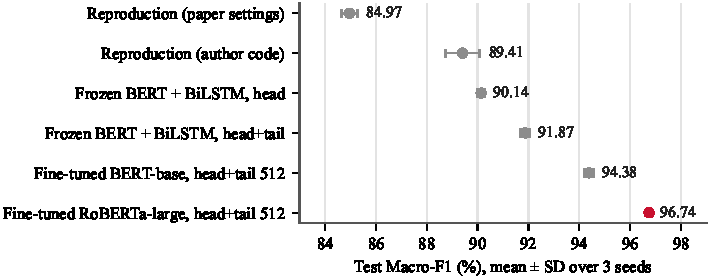
\includegraphics[width=\columnwidth]{fig_progression}
\caption{Test Macro-F1 of the main configurations. Error bars show the standard deviation over three seeds; for most systems they are smaller than the marker.}
\label{fig:progression}
\end{figure}

\subsection{From frozen features to fine-tuning}
Fig.~\ref{fig:progression} summarizes the progression. With a frozen encoder, replacing mean pooling by a BiLSTM adds 4.43 points (85.71\% to 90.14\%), which confirms that the recurrent head extracts useful order information from the token states. Our frozen BiLSTM over the first 256 tokens is 0.73 points better than the reproduction of the author code. The two differ in the optimizer (AdamW), in skipping padding through packed sequences, in training length (50 epochs) and in validation-based checkpoint selection; we did not ablate these factors individually.

Changing only the input selection, from the first 256 tokens to head plus tail, adds another 1.73 points (91.87\%). Fine-tuning the whole BERT-base encoder on 512 head--tail tokens adds 2.51 points more (94.38\%), and replacing BERT-base by RoBERTa-large adds 2.37 points (96.74\%). RoBERTa-large is also the most stable configuration, with a standard deviation of 0.04 points across seeds.

\subsection{Where the gains come from}
Fig.~\ref{fig:length}(a) splits the frozen BiLSTM results by review length. On short reviews, which are not affected by the input selection, head--tail and head-only inputs perform almost identically (92.9\% vs.\ 92.4\%). On the 10{,}026 truncated test reviews, head--tail inputs raise Macro-F1 from 86.7\% to 90.3\%. The improvement is therefore concentrated where the head-only model discards the end of the review, which supports the intuition that the closing sentences often carry the reviewer's verdict.

Fig.~\ref{fig:length}(b) repeats the analysis for the fine-tuned models, where a review is truncated if it exceeds 512 tokens. BERT-base still loses about one point on truncated reviews (93.6\% vs.\ 94.5\%). RoBERTa-large does not: its Macro-F1 on the 2{,}940 truncated reviews (96.9\%) is as high as on short reviews (96.7\%). With a sufficiently strong encoder, discarding the middle of very long reviews no longer costs accuracy on this task.

\begin{figure}[t]
\centering
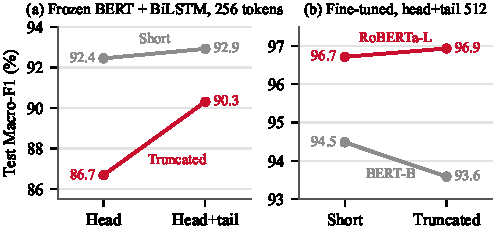
\includegraphics[width=\columnwidth]{fig_length}
\caption{Test Macro-F1 by review length (mean over three seeds). (a) Frozen BERT with a BiLSTM head; truncated means longer than 256 tokens. (b) Fine-tuned models with head--tail inputs; truncated means longer than 512 tokens for the respective tokenizer.}
\label{fig:length}
\end{figure}

\subsection{Per-seed behaviour and error balance}
Table~\ref{tab:seeds} lists the individual runs together with the number of false positives (negative reviews predicted positive) and false negatives. The code reproduction is not only less accurate but also unstable in a specific way: its decision bias changes from seed to seed. Seed 42 produces three times more false positives than false negatives, while seed 44 produces almost twice as many false negatives as false positives. The paper configuration is biased towards the positive class in all three runs. In contrast, both fine-tuned models make far more balanced errors, and RoBERTa-large is almost perfectly balanced in every run. Pooled over the three seeds, RoBERTa-large reaches a precision of 96.90\% and a recall of 96.58\% on the negative class, and a precision of 96.59\% and a recall of 96.91\% on the positive class, so its remaining errors are not explained by a systematic preference for one label.

\begin{table}[t]
\caption{Individual test runs: Macro-F1 (\%), false positives (FP) and false negatives (FN)}
\label{tab:seeds}
\centering
\footnotesize
\setlength{\tabcolsep}{2.2pt}
\begin{tabular}{lrrrrrrrrr}
\toprule
 & \multicolumn{3}{c}{Seed 42} & \multicolumn{3}{c}{Seed 43} & \multicolumn{3}{c}{Seed 44} \\
\cmidrule(lr){2-4}\cmidrule(lr){5-7}\cmidrule(lr){8-10}
System & F1 & FP & FN & F1 & FP & FN & F1 & FP & FN \\
\midrule
Repro (paper) & 85.13 & 2161 & 1555 & 84.62 & 2747 & 1082 & 85.15 & 2420 & 1284 \\
Repro (code) & 88.81 & 2118 & 670 & 90.13 & 1170 & 1297 & 89.29 & 933 & 1741 \\
Frozen h+t & 91.79 & 943 & 1109 & 91.76 & 1091 & 968 & 92.06 & 971 & 1013 \\
BERT-B FT & 94.18 & 632 & 822 & 94.47 & 708 & 674 & 94.47 & 837 & 545 \\
RoBERTa-L FT & 96.71 & 433 & 390 & 96.74 & 450 & 365 & 96.78 & 401 & 404 \\
\bottomrule
\multicolumn{10}{l}{\scriptsize Each test set contains 12{,}500 negative and 12{,}500 positive reviews.}
\end{tabular}
\end{table}

\subsection{Statistical significance}
Table~\ref{tab:sig} and Fig.~\ref{fig:sig} report the eight planned comparisons. All 95\% confidence intervals exclude zero, and all Holm-adjusted bootstrap $p$-values are at the floor of 0.0016 imposed by the number of resamples. The per-seed McNemar tests agree for every comparison except the smallest one: the frozen head-only BiLSTM versus the code reproduction is significant for seeds 42 and 44 but not for seed 43 ($p=0.94$), so that 0.73-point difference should be read with caution. All differences of two points or more are significant under both tests, with McNemar $p<10^{-18}$ for every seed.

\begin{table}[t]
\caption{Paired comparisons of test Macro-F1 (points)}
\label{tab:sig}
\centering
\footnotesize
\setlength{\tabcolsep}{3pt}
\begin{tabular}{lccc}
\toprule
Comparison & $\Delta$ & 95\% CI & Max McNemar $p$ \\
\midrule
RoBERTa-L FT vs BERT-B FT & +2.37 & [2.14, 2.60] & $3\times10^{-67}$ \\
RoBERTa-L FT vs frozen h+t & +4.87 & [4.56, 5.19] & $1\times10^{-188}$ \\
RoBERTa-L FT vs repro (code) & +7.33 & [6.95, 7.72] & $1\times10^{-292}$ \\
BERT-B FT vs frozen h+t & +2.50 & [2.24, 2.76] & $2\times10^{-49}$ \\
BERT-B FT vs repro (code) & +4.96 & [4.65, 5.28] & $3\times10^{-135}$ \\
BERT-B FT vs repro (paper) & +9.41 & [8.97, 9.85] & $<10^{-300}$ \\
Frozen h+t vs repro (code) & +2.46 & [2.18, 2.75] & $5\times10^{-19}$ \\
Frozen head vs repro (code) & +0.73 & [0.53, 0.93] & 0.94 \\
\bottomrule
\multicolumn{4}{l}{\footnotesize Holm-adjusted bootstrap $p\le0.0016$ (the floor) for all rows.}
\end{tabular}
\end{table}

\begin{figure}[t]
\centering
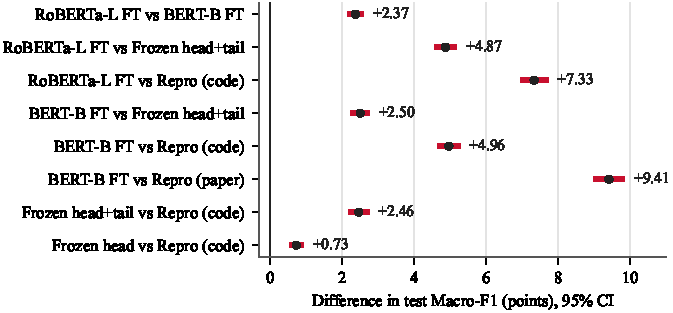
\includegraphics[width=\columnwidth]{fig_significance}
\caption{Differences in test Macro-F1 with 95\% confidence intervals from a paired bootstrap over 3{,}581 test movies (10{,}000 resamples).}
\label{fig:sig}
\end{figure}

\subsection{Training dynamics}
Fig.~\ref{fig:validation} shows validation Macro-F1 after each epoch. For BERT-base, all three seeds peak after the second epoch and decline slightly in the third, which indicates the onset of over-fitting; validation-based selection picks epoch 2 in every case. RoBERTa-large improves more steadily, and the selected epoch is 3 for two seeds and 2 for one. In both cases the test results of the selected checkpoints are tightly clustered.

\begin{figure}[t]
\centering
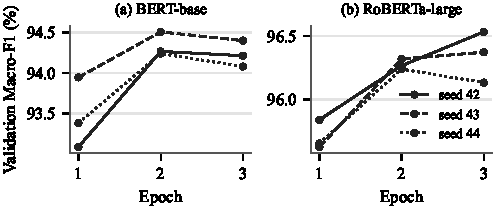
\includegraphics[width=\columnwidth]{fig_validation}
\caption{Validation Macro-F1 after each epoch of fine-tuning for the three seeds.}
\label{fig:validation}
\end{figure}

\subsection{Qualitative error analysis}
To understand the remaining errors of the frozen models, we read 100 validation reviews in full: 40 misclassified by both the head-only and the head--tail BiLSTM, 20 corrected by head--tail inputs, 20 broken by them and 20 classified correctly by both. The sample was stratified by label and length rather than drawn at random, and the annotations were made by a single annotator, so the counts below describe the sample, not the dataset. Four recurring patterns explain most errors. In 9 cases the reviewer enjoys a film for being bad, uses sarcasm, or judges it against genre conventions; reading more text does not resolve these, because they require pragmatic inference. In 6 cases the review praises or criticizes a \emph{different} film used as a comparison. In 4 long reviews the verdict is a single sentence buried in a plot summary, which neither truncation strategy reliably keeps. Finally, 2 records are not reviews at all (posting instructions and gossip), and 6 reviews appear inconsistent with their label; we flag the latter for inspection but keep all labels unchanged.

\section{Discussion}
\textit{Comparability.} The accuracy of our reproduced baseline (89.43\%) is 8.2 points below the accuracy reported in~\cite{nkhata2023}. Because the original evaluation used a different split, this gap does not show that the original number is wrong; it shows that results obtained on re-split IMDb data should not be compared with results on the official test set. We recommend that future work on IMDb either keeps the official split or publishes its split together with the code.

\textit{What matters most.} Two simple changes account for most of the improvement: keeping the end of long reviews and letting the encoder adapt to the task. Each of them is visible in isolation (Fig.~\ref{fig:length}a and the gap between frozen and fine-tuned models), and both are inexpensive compared with architectural changes to the classification head.

\textit{Cost.} RoBERTa-large is about three times larger than BERT-base and needs gradient checkpointing to fit in 8~GB of memory. Where resources are tight, fine-tuned BERT-base with head--tail inputs offers most of the gain (94.38\%) at a fraction of the cost. We did not measure inference latency.

\textit{Recommendations.} Our experience suggests a short checklist for reproducing text classifiers on IMDb and similar corpora: (i) evaluate on the official test split, or publish the split used; (ii) remove duplicates and cross-split leakage before training and report how many reviews were removed; (iii) report the fraction of inputs that exceed the model's length limit and how they were truncated; (iv) select checkpoints on a validation set only; (v) report the mean and variance over several seeds; and (vi) test differences with a method that respects the dependence between reviews of the same movie.

\textit{Limitations.} All results come from one dataset in one language with binary labels, and three seeds per configuration give a reasonable but limited view of run-to-run variance. Part of the official test set (reviews of horror movies) was inspected during an earlier phase of this project, so the test set is not entirely unseen, although no hyper-parameter or threshold was tuned on it. Finally, the training times we report were measured on a shared laptop GPU and are not a controlled benchmark.

\textit{Future work.} Natural next steps are domain-adaptive masked language modeling on IMDb text~\cite{gururangan2020}, ensembles of the fine-tuned models, encoders that read whole long documents such as Longformer~\cite{beltagy2020}, and an evaluation on Vietnamese translations of the reviews.

\section{Conclusion}
We reproduced a BERT+BiLSTM sentiment classifier on a leakage-controlled IMDb split and obtained 89.41\% test Macro-F1 for the configuration of the released code, compared with the 97.67\% accuracy reported on a re-split of the data. We showed that truncation of long reviews is the main weakness of that pipeline, and that keeping the head and the tail of each review together with full fine-tuning removes most of it. Fine-tuned RoBERTa-large with 512 head--tail tokens reaches 96.74\%$\pm$0.04 Macro-F1, 7.33 points above the reproduced baseline, and the improvement is statistically significant under a movie-clustered bootstrap and McNemar tests.

\section*{Acknowledgment}
We thank the authors of~\cite{nkhata2023} for releasing their code, and Maas \textit{et al.} for the IMDb dataset.

\begin{thebibliography}{00}
\bibitem{maas2011} A. L. Maas, R. E. Daly, P. T. Pham, D. Huang, A. Y. Ng, and C. Potts, ``Learning word vectors for sentiment analysis,'' in \textit{Proc. 49th Annu. Meeting Assoc. Comput. Linguistics: Human Language Technologies}, Portland, OR, USA, 2011, pp. 142--150.
\bibitem{devlin2019} J. Devlin, M.-W. Chang, K. Lee, and K. Toutanova, ``BERT: Pre-training of deep bidirectional transformers for language understanding,'' in \textit{Proc. NAACL-HLT}, 2019, pp. 4171--4186.
\bibitem{liu2019roberta} Y. Liu \textit{et al.}, ``RoBERTa: A robustly optimized BERT pretraining approach,'' arXiv:1907.11692, 2019.
\bibitem{nkhata2023} G. Nkhata, S. Gauch, U. Anjum, and J. Zhan, ``Fine-tuning BERT with bidirectional LSTM for fine-grained movie reviews sentiment analysis,'' \textit{Int. J. Advances in Systems and Measurements}, vol. 16, no. 3--4, 2023; arXiv:2502.20682.
\bibitem{hochreiter1997} S. Hochreiter and J. Schmidhuber, ``Long short-term memory,'' \textit{Neural Computation}, vol. 9, no. 8, pp. 1735--1780, 1997.
\bibitem{schuster1997} M. Schuster and K. K. Paliwal, ``Bidirectional recurrent neural networks,'' \textit{IEEE Trans. Signal Process.}, vol. 45, no. 11, pp. 2673--2681, 1997.
\bibitem{sun2019} C. Sun, X. Qiu, Y. Xu, and X. Huang, ``How to fine-tune BERT for text classification?'' in \textit{Proc. China National Conf. Chinese Computational Linguistics (CCL)}, 2019, pp. 194--206.
\bibitem{kim2014} Y. Kim, ``Convolutional neural networks for sentence classification,'' in \textit{Proc. Conf. Empirical Methods in Natural Language Processing (EMNLP)}, 2014, pp. 1746--1751.
\bibitem{yang2016han} Z. Yang, D. Yang, C. Dyer, X. He, A. Smola, and E. Hovy, ``Hierarchical attention networks for document classification,'' in \textit{Proc. NAACL-HLT}, 2016, pp. 1480--1489.
\bibitem{howard2018} J. Howard and S. Ruder, ``Universal language model fine-tuning for text classification,'' in \textit{Proc. 56th Annu. Meeting Assoc. Comput. Linguistics}, 2018, pp. 328--339.
\bibitem{pappagari2019} R. Pappagari, P. Żelasko, J. Villalba, Y. Carmiel, and N. Dehak, ``Hierarchical transformers for long document classification,'' in \textit{Proc. IEEE Automatic Speech Recognition and Understanding Workshop (ASRU)}, 2019, pp. 838--844.
\bibitem{beltagy2020} I. Beltagy, M. E. Peters, and A. Cohan, ``Longformer: The long-document transformer,'' arXiv:2004.05150, 2020.
\bibitem{dodge2019} J. Dodge, S. Gururangan, D. Card, R. Schwartz, and N. A. Smith, ``Show your work: Improved reporting of experimental results,'' in \textit{Proc. EMNLP-IJCNLP}, 2019, pp. 2185--2194.
\bibitem{efron1993} B. Efron and R. J. Tibshirani, \textit{An Introduction to the Bootstrap}. New York, NY, USA: Chapman \& Hall, 1993.
\bibitem{holm1979} S. Holm, ``A simple sequentially rejective multiple test procedure,'' \textit{Scandinavian J. Statistics}, vol. 6, no. 2, pp. 65--70, 1979.
\bibitem{mcnemar1947} Q. McNemar, ``Note on the sampling error of the difference between correlated proportions or percentages,'' \textit{Psychometrika}, vol. 12, no. 2, pp. 153--157, 1947.
\bibitem{dietterich1998} T. G. Dietterich, ``Approximate statistical tests for comparing supervised classification learning algorithms,'' \textit{Neural Computation}, vol. 10, no. 7, pp. 1895--1923, 1998.
\bibitem{paszke2019} A. Paszke \textit{et al.}, ``PyTorch: An imperative style, high-performance deep learning library,'' in \textit{Advances in Neural Information Processing Systems 32}, 2019.
\bibitem{wolf2020} T. Wolf \textit{et al.}, ``Transformers: State-of-the-art natural language processing,'' in \textit{Proc. EMNLP: System Demonstrations}, 2020, pp. 38--45.
\bibitem{loshchilov2019} I. Loshchilov and F. Hutter, ``Decoupled weight decay regularization,'' in \textit{Proc. Int. Conf. Learning Representations (ICLR)}, 2019.
\bibitem{chen2016} T. Chen, B. Xu, C. Zhang, and C. Guestrin, ``Training deep nets with sublinear memory cost,'' arXiv:1604.06174, 2016.
\bibitem{gururangan2020} S. Gururangan \textit{et al.}, ``Don't stop pretraining: Adapt language models to domains and tasks,'' in \textit{Proc. 58th Annu. Meeting Assoc. Comput. Linguistics}, 2020, pp. 8342--8360.
\end{thebibliography}

\end{document}
